\documentclass[border=3pt,tikz]{standalone}

% define the angle so that 2theta = pi/7
\def\theta{12.86}

% define the circles of radius 1, 2, 3
\def\shapeA{(0,0) circle (1cm)}
\def\shapeB{(0,0) circle (2cm)}
\def\shapeC{(0,0) circle (3cm)}

% define the intersecting lines
\def\shapeD{(-\theta:3.5cm) -- (0,0) -- (\theta:3.5cm)}
\def\shapeE{(180+\theta:3.5cm) -- (0,0) -- (180-\theta:3.5cm)}

\begin{document}

% scope the fill with a \clip \shapeC: inside the scope environment, nothing is drawn outside of shapeC.
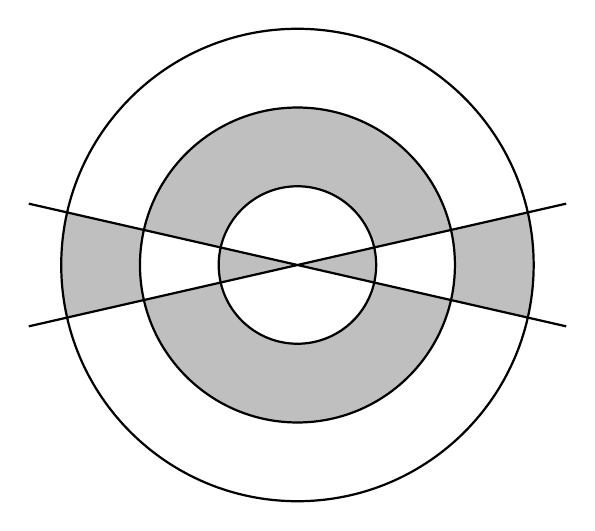
\begin{tikzpicture}[thick]
    \begin{scope}
        \clip \shapeC;
        \fill[fill=lightgray, even odd rule]  \shapeE \shapeB \shapeD \shapeA;
    \end{scope}
  
  \draw \shapeA \shapeB \shapeC \shapeD \shapeE;
\end{tikzpicture}

\end{document}